\documentclass[
	classe=$2^{de}$,
]{exercice}

\usepackage{tkz-tab}
\usetikzlibrary{calc}

\renewcommand{\arraystretch}{1.3}
\newcommand{\computeF}[1]{
	\pgfmathparse{int(0.5*#1*#1 + 0.5*(10-#1)*(10-#1))}
	\pgfmathresult
}

\title{Exercice : aire de deux triangles}

\begin{document}

\maketitle

On considère la figure suivante, où $AB = 10$cm, et $M$ est un point mobile :

\begin{center}
	\begin{tikzpicture}
		\pgfmathsetmacro\x{6}
		\coordinate (A) at (0,0);
		\coordinate (B) at (10,0);
		\coordinate (M) at (\x,0);
		\coordinate (N) at ($(A) + (0,\x)$);
		\coordinate (P) at ($(M) + (0,10-\x)$);

		\foreach \p/\dir in {A/below,B/below,M/below,N/above left,P/above left} {
				\node[\dir] at (\p) {\p};
			}
		\draw (A) -- (B) -- (P) -- (M) -- (N) -- (A);

		\draw[<->] ($(A) + (0,-0.7)$) -- node[midway,below] {$x$} ($(M) + (0,-0.7)$);
	\end{tikzpicture}
\end{center}

On appelle $x$ la distance $AM$, et on définit la fonction $f(x) = $ Aire($AMN$) + Aire($MBP$).

On va alors chercher à minimiser la valeur de $f(x)$.

\begin{enumerate}
	\item Quelle est la valeur de $f(x)$ si $x = 0$cm ? \correction{$f(0) = 10 × 10 ÷ 2 = 50$cm$²$}
	\item Quelle est la valeur de $f(x)$ si $x = 2$cm ? \correction{$f(2) = (8² + 2²) ÷ 2 = 34$cm$²$}
	\item Donner l'expression de la fonction $f$ :

	      $$ f(x) = \correctionDots{\dfrac{x^2 + (10-x)^2}{2}} $$
	\item Remplir le tableau suivant :
	      \begin{center}
		      \begin{tabular}{|l|*{11}{>{\centering}p{0.8cm}|}}
			      \hline
			      $x$    & $0$                         & $1$                         & $2$                         & $3$                         & $4$                         & $5$                         & $6$                         & $7$                         & $8$                         & $9$                         & $10$                         \tabularnewline \hline
			      $f(x)$ & $\correction{\computeF{0}}$ & $\correction{\computeF{1}}$ & $\correction{\computeF{2}}$ & $\correction{\computeF{3}}$ & $\correction{\computeF{4}}$ & $\correction{\computeF{5}}$ & $\correction{\computeF{6}}$ & $\correction{\computeF{7}}$ & $\correction{\computeF{8}}$ & $\correction{\computeF{9}}$ & $\correction{\computeF{10}}$ \tabularnewline \hline
		      \end{tabular}
	      \end{center}
	\item On voit que
	      \begin{itemize}
		      \item $f$ est décroissante entre $\correctionDots{\phantom{1}0}$ et $\correctionDots{\phantom{1}5}$.
		      \item $f$ est croissante entre $\correctionDots{\phantom{1}5}$ et $\correctionDots{10}$.
	      \end{itemize}
	      Remplir alors le tableau de variations de $f$ :

	      \begin{center}
		      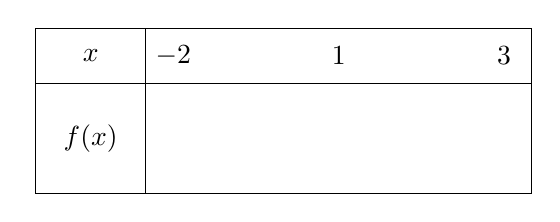
\begin{tikzpicture}[scale=0.7]
			      \tkzTabInit{$x$ / 1 , $f(x)$ / 2}{$\correction{-2}$, $\correction{1}$, $\correction{3}$}
			      \ifdefined\makeCorrection
				      \color{red}
				      \tkzTabVar{+/ $7$, -/ $-2$, +/ $2$}
			      \fi
		      \end{tikzpicture}
	      \end{center}
\end{enumerate}

\end{document}